% 第三部分 B：结果（由 main_zh.tex 引入）。

\section{结果}\label{sec:res}

每个条件跑了 \NUM{seeds_subkev} 个种子，各 200 步；第二部分给每个解答都打标签的 \texttt{rlvr} 是满标注预算的参照（\NUM{seeds_rlvr} 个种子）。表~\ref{tab:sub-acc} 给出最终策略的准确率，表~\ref{tab:sub-seeds} 给出每个 run 的准确率，表~\ref{tab:sub-paired} 给出相对 \texttt{rlvr\_sub}（直接丢掉未标注解答的条件）的配对差。表~\ref{tab:sub-fill} 给出每种补全奖励在它所打分的解答上有多准，表~\ref{tab:sub-style} 给出每个最终策略写了什么，图~\ref{fig:sub-curves} 给出训练曲线。区间按题目重采样，不包含种子之间的差异；在本项目的 GRPO run 中，种子之间的差异可能大于条件之间的差异（第二部分 \S8）。

\begin{table}[t]
\centering\small
\begin{tabular}{@{}lcccccc@{}}
\toprule
condition & seeds & MATH-500 & GSM8K & AMC23 & AIME24 & AIME25 \\ \midrule
base model & -- & 76.5 & 87.9 & 50.6 & 10.0 & 10.9 \\ \midrule
\texttt{rlvr} & 3 & 82.5 $\pm$ 0.6 & 93.0 $\pm$ 0.3 & 60.9 $\pm$ 2.4 & 21.5 $\pm$ 0.4 & 16.7 $\pm$ 2.1 \\
\texttt{rlvr\_sub} & 2 & 81.8 $\pm$ 1.7 & 92.4 $\pm$ 0.4 & 60.8 $\pm$ 1.1 & 18.3 $\pm$ 1.8 & 15.4 $\pm$ 0.3 \\
\texttt{sub\_kev} & 2 & 79.5 $\pm$ 1.3 & 91.2 $\pm$ 1.3 & 56.1 $\pm$ 3.5 & 15.9 $\pm$ 1.6 & 14.5 $\pm$ 1.6 \\
\texttt{sub\_kev\_recal} & 2 & 81.2 $\pm$ 2.5 & 92.3 $\pm$ 0.9 & 59.4 $\pm$ 1.8 & 21.1 $\pm$ 4.6 & 14.7 $\pm$ 3.4 \\
\texttt{sub\_probe} & 2 & 85.9 $\pm$ 1.8 & 93.7 $\pm$ 0.5 & 67.7 $\pm$ 2.3 & 30.5 $\pm$ 0.1 & 23.9 $\pm$ 1.3 \\
\bottomrule
\end{tabular}

\caption{最终策略：准确率（\%），种子均值 $\pm$ 种子间标准差。MATH-500 和 GSM8K：贪心解码。AMC23、AIME24 和 AIME25：温度 0.6 下每题 16 个样本的平均。\texttt{rlvr}：每个解答都打标签（第二部分）；其他条件每组 8 个解答只标注 2 个。}
\label{tab:sub-acc}
\end{table}

\begin{table}[t]
\centering\small
\begin{tabular}{@{}lcccccc@{}}
\toprule
condition & seed & MATH-500 & GSM8K & AMC23 & AIME24 & AIME25 \\ \midrule
\texttt{rlvr} & 1 & 82.8 & 93.0 & 63.6 & 21.0 & 18.8 \\
 & 2 & 83.0 & 93.3 & 59.8 & 21.9 & 16.9 \\
 & 3 & 81.8 & 92.6 & 59.2 & 21.7 & 14.6 \\
\addlinespace
\texttt{rlvr\_sub} & 1 & 80.6 & 92.6 & 61.6 & 19.6 & 15.6 \\
 & 2 & 83.0 & 92.1 & 60.0 & 17.1 & 15.2 \\
\addlinespace
\texttt{sub\_kev} & 1 & 78.6 & 90.3 & 53.6 & 14.8 & 13.3 \\
 & 2 & 80.4 & 92.1 & 58.6 & 17.1 & 15.6 \\
\addlinespace
\texttt{sub\_kev\_recal} & 1 & 79.4 & 91.7 & 58.1 & 17.9 & 12.3 \\
 & 2 & 83.0 & 92.9 & 60.6 & 24.4 & 17.1 \\
\addlinespace
\texttt{sub\_probe} & 1 & 87.2 & 93.3 & 69.4 & 30.6 & 22.9 \\
 & 2 & 84.6 & 94.1 & 66.1 & 30.4 & 24.8 \\
\bottomrule
\end{tabular}

\caption{每个 run 的最终策略：准确率（\%），口径同表~\ref{tab:sub-acc}。}
\label{tab:sub-seeds}
\end{table}

\paragraph{丢掉四分之三的标签，代价不大。} 每组只用两个已标注解答时，\texttt{rlvr\_sub} 在 MATH-500 上达到 \NUM{acc_sub_math}\%（两个种子为 \NUM{acc_sub_math_s1}\% 和 \NUM{acc_sub_math_s2}\%）。八个都标注（\texttt{rlvr}）多出 \NUM{d_rlvr_math} \ci{\NUM{dlo_rlvr_math}}{\NUM{dhi_rlvr_math}} 个百分点，AIME24 上多出 \NUM{d_rlvr_aime24} \ci{\NUM{dlo_rlvr_aime24}}{\NUM{dhi_rlvr_aime24}}。补全奖励能挽回的就是这么多——前提是它不教给策略别的东西。

\begin{table}[t]
\centering\small
\begin{tabular}{@{}lccccc@{}}
\toprule
minus \texttt{rlvr\_sub} & MATH-500 & GSM8K & AMC23 & AIME24 & AIME25 \\ \midrule
\texttt{rlvr} & $+$0.7 & $+$0.6 & $+$0.1 & $+$3.2 & $+$1.3 \\
 & {\footnotesize \ci{$-$1.1}{2.7}} & {\footnotesize \ci{$-$0.2}{1.4}} & {\footnotesize \ci{$-$3.2}{3.3}} & {\footnotesize \ci{1.0}{5.7}} & {\footnotesize \ci{$-$0.7}{3.3}} \\[2pt]
\texttt{sub\_kev} & $-$2.3 & $-$1.2 & $-$4.7 & $-$2.4 & $-$0.9 \\
 & {\footnotesize \ci{$-$4.4}{$-$0.1}} & {\footnotesize \ci{$-$2.1}{$-$0.2}} & {\footnotesize \ci{$-$8.8}{$-$0.3}} & {\footnotesize \ci{$-$5.3}{0.1}} & {\footnotesize \ci{$-$4.2}{2.2}} \\[2pt]
\texttt{sub\_kev\_recal} & $-$0.6 & $+$0.0 & $-$1.4 & $+$2.8 & $-$0.7 \\
 & {\footnotesize \ci{$-$2.8}{1.6}} & {\footnotesize \ci{$-$0.9}{0.8}} & {\footnotesize \ci{$-$5.5}{3.2}} & {\footnotesize \ci{0.8}{5.2}} & {\footnotesize \ci{$-$3.1}{1.4}} \\[2pt]
\texttt{sub\_probe} & $+$4.1 & $+$1.3 & $+$7.0 & $+$12.2 & $+$8.4 \\
 & {\footnotesize \ci{1.6}{6.6}} & {\footnotesize \ci{0.4}{2.3}} & {\footnotesize \ci{2.7}{11.2}} & {\footnotesize \ci{5.2}{20.3}} & {\footnotesize \ci{4.0}{13.5}} \\[2pt]
\bottomrule
\end{tabular}

\caption{相对 \texttt{rlvr\_sub} 的配对差（百分点）：逐题取各条件的种子均值之差，再对题目取平均，附按题目自助法得到的 95\% 区间。}
\label{tab:sub-paired}
\end{table}

\paragraph{冻结的评判模型让结果更差。} 用发布版 \kev{} 的 $\pc$ 给未标注解答打分（\texttt{sub\_kev}），两个种子都比直接丢掉它们差（MATH-500 上 \NUM{acc_subkev_math_s1}\% 和 \NUM{acc_subkev_math_s2}\%）：MATH-500 上差 \NUM{d_subkev_math} \ci{\NUM{dlo_subkev_math}}{\NUM{dhi_subkev_math}} 个百分点，AMC23 上差 \NUM{d_subkev_amc} \ci{\NUM{dlo_subkev_amc}}{\NUM{dhi_subkev_amc}}，AIME24 上差 \NUM{d_subkev_aime24} \ci{\NUM{dlo_subkev_aime24}}{\NUM{dhi_subkev_aime24}}。然而评判模型对未标注解答的排序一直很好：它对被隐去标签的 AUROC 在整个 run 上为 \NUM{fillauc_all_subkev}（表~\ref{tab:sub-fill}）。问题在于它太慷慨：前 20 步它在未标注解答上的平均 $\pc$ 为 \NUM{fillmean_first20_subkev}，而其中只有 \NUM{unlacc_first20_subkev}\% 正确；最后 20 步为 \NUM{fillmean_last20_subkev}，正确的有 \NUM{unlacc_last20_subkev}\%。哪些解答被标注是随机的，所以一个常数偏移会让每种行为的期望奖励提高同样的量，组基线在期望上会把它消掉。但一个为某种行为付出超出其正确性所值的回报的评判模型，会改变策略学到的东西。两个策略都学会了重复自己：它们的 MATH-500 解答中分别有 \NUM{srep_subkev_s1} 和 \NUM{srep_subkev_s2} 的行与前面某行相同，\texttt{rlvr\_sub} 为 \NUM{srep_sub_s1} 和 \NUM{srep_sub_s2}；种子 1 有 \NUM{strunc_subkev_s1} 的解答写到 2048 词元的上限（表~\ref{tab:sub-style}）。在第一个答案之后，种子 1 一遍又一遍地重述结论，常常一直写到长度上限；种子 2 则把题目再解一遍。两者都不改变验证器读到的答案，所以已标注的解答不会惩罚这种行为，而在未标注的解答上评判模型会为它付费（\S\ref{sec:res-repeat}）。

\begin{table}[t]
\centering\small
\begin{tabular}{@{}lcccccccc@{}}
\toprule
 & & \multicolumn{3}{c}{fill-in AUROC} & frozen \kev{} & & \multicolumn{2}{c}{mean} \\ \cmidrule(lr){3-5}\cmidrule(l){8-9}
condition & seeds & steps 0--19 & first half & second half & AUROC & ECE & fill-in & label \\ \midrule
\texttt{sub\_kev} & 2 & 0.89 & 0.92 & 0.90 & 0.91 & 0.19 & 0.75 & 0.60 \\
\texttt{sub\_kev\_recal} & 2 & 0.92 & 0.94 & 0.92 & 0.90 & 0.10 & 0.63 & 0.62 \\
\texttt{sub\_probe} & 2 & 0.93 & 0.95 & 0.92 & 0.91 & 0.11 & 0.66 & 0.65 \\
\bottomrule
\end{tabular}

\caption{补全奖励在未标注解答上对照验证器被隐去的标签（逐步计算，再对步数和种子取平均）：前 20 步与 run 前后两半的 AUROC、冻结 \kev{} 在同样解答上的 AUROC、期望校准误差，以及平均补全奖励与其中正确解答所占比例的对照。}
\label{tab:sub-fill}
\end{table}

\paragraph{重新校准修正了校准，没有修正偏好。} 在迄今收集的标签上重新拟合 \kev{} 的输出头（\texttt{sub\_kev\_recal}），在它被拟合的那些数上如预期般起作用：它在未标注解答上的校准误差为 \NUM{fillece_all_subrecal}（冻结输出头为 \NUM{fillece_all_subkev}），平均补全奖励 \NUM{fillmean_all_subrecal} 与其中 \NUM{unlacc_all_subrecal}\% 的正确率相符，在同样的解答上排序也略好于冻结输出头（AUROC \NUM{fillauc_all_subrecal} 对 \NUM{frozenauc_all_subrecal}）。种子 1 仍然学会了重复自己（\NUM{srep_subrecal_s1} 的行），MATH-500 最终为 \NUM{acc_subrecal_math_s1}\%；种子 2 没有（\NUM{srep_subrecal_s2}），最终为 \NUM{acc_subrecal_math_s2}\%。两个种子合起来，这个条件并不比丢掉未标注解答更好（MATH-500 上 \NUM{d_subrecal_math} \ci{\NUM{dlo_subrecal_math}}{\NUM{dhi_subrecal_math}}）。

\paragraph{从头训练的输出头：两个种子都改成了先写草稿。} 探针（\texttt{sub\_probe}）的排序和校准与重新校准的输出头大致相当（AUROC \NUM{fillauc_all_subprobe}，校准误差 \NUM{fillece_all_subprobe}），它的两个策略都不重复自己（分别 \NUM{srep_subprobe_s1} 和 \NUM{srep_subprobe_s2} 的行）。两者最终都远高于本文其他所有 run：MATH-500 上 \NUM{acc_subprobe_math_s1}\% 和 \NUM{acc_subprobe_math_s2}\%，AIME24 上 \NUM{acc_subprobe_aime24_s1}\% 和 \NUM{acc_subprobe_aime24_s2}\%。两个种子合起来，在 MATH-500 上比 \texttt{rlvr\_sub} 高 \NUM{d_subprobe_math} \ci{\NUM{dlo_subprobe_math}}{\NUM{dhi_subprobe_math}} 个百分点，在 AIME24 上高 \NUM{d_subprobe_aime24} \ci{\NUM{dlo_subprobe_aime24}}{\NUM{dhi_subprobe_aime24}}，也高于满标注的 \texttt{rlvr}（MATH-500 上 \NUM{acc_rlvr_math}\%）。两个策略的写法都与众不同：先用纯文本把题目做一遍，其中分别有 \NUM{sdraftfmt_subprobe_s1} 和 \NUM{sdraftfmt_subprobe_s2} 的草稿之后再写格式化的解答（\S\ref{sec:res-style}）。

\begin{table}[t]
\centering\small
\setlength{\tabcolsep}{4.5pt}
\begin{tabular}{@{}lccccccccc@{}}
\toprule
 & & & & \multicolumn{2}{c}{repeated lines} & several & draft & \multicolumn{2}{c}{\kev{} $\pc$} \\ \cmidrule(lr){5-6}\cmidrule(l){9-10}
condition & seed & tokens & truncated & share & after answer & answers & opening & right & wrong \\ \midrule
\texttt{rlvr} & 1 & 541 & 2\% & 1\% & 0\% & 2\% & 1\% & 0.84 & 0.60 \\
 & 2 & 555 & 4\% & 1\% & 0\% & 6\% & 0\% & 0.85 & 0.59 \\
 & 3 & 909 & 8\% & 28\% & 90\% & 95\% & 1\% & 0.88 & 0.64 \\
\addlinespace
\texttt{rlvr\_sub} & 1 & 630 & 6\% & 1\% & 0\% & 3\% & 1\% & 0.84 & 0.54 \\
 & 2 & 588 & 3\% & 1\% & 0\% & 3\% & 2\% & 0.83 & 0.56 \\
\addlinespace
\texttt{sub\_kev} & 1 & 1723 & 69\% & 49\% & 49\% & 99\% & 1\% & 0.91 & 0.72 \\
 & 2 & 1072 & 12\% & 24\% & 85\% & 97\% & 2\% & 0.91 & 0.71 \\
\addlinespace
\texttt{sub\_kev\_recal} & 1 & 904 & 3\% & 22\% & 85\% & 98\% & 7\% & 0.90 & 0.71 \\
 & 2 & 538 & 3\% & 1\% & 0\% & 11\% & 1\% & 0.85 & 0.62 \\
\addlinespace
\texttt{sub\_probe} & 1 & 546 & 6\% & 0\% & 0\% & 75\% & 90\% & 0.90 & 0.61 \\
 & 2 & 694 & 6\% & 0\% & 0\% & 71\% & 90\% & 0.91 & 0.66 \\
\bottomrule
\end{tabular}

\caption{每个最终策略在 MATH-500 上写了什么（贪心）：解答词元数、在 2048 词元处被截断的比例、（至少 20 个字符的）行与同一解答前面某行相同的比例、在第一个框出答案之后重复这样一行的解答比例、含有多个框出答案的解答比例（验证器读最后一个）、以非正式草稿开头的解答比例，以及 \kev{} 对正确与错误答案的 $\pc$。}
\label{tab:sub-style}
\end{table}

\begin{figure}[t]
\centering
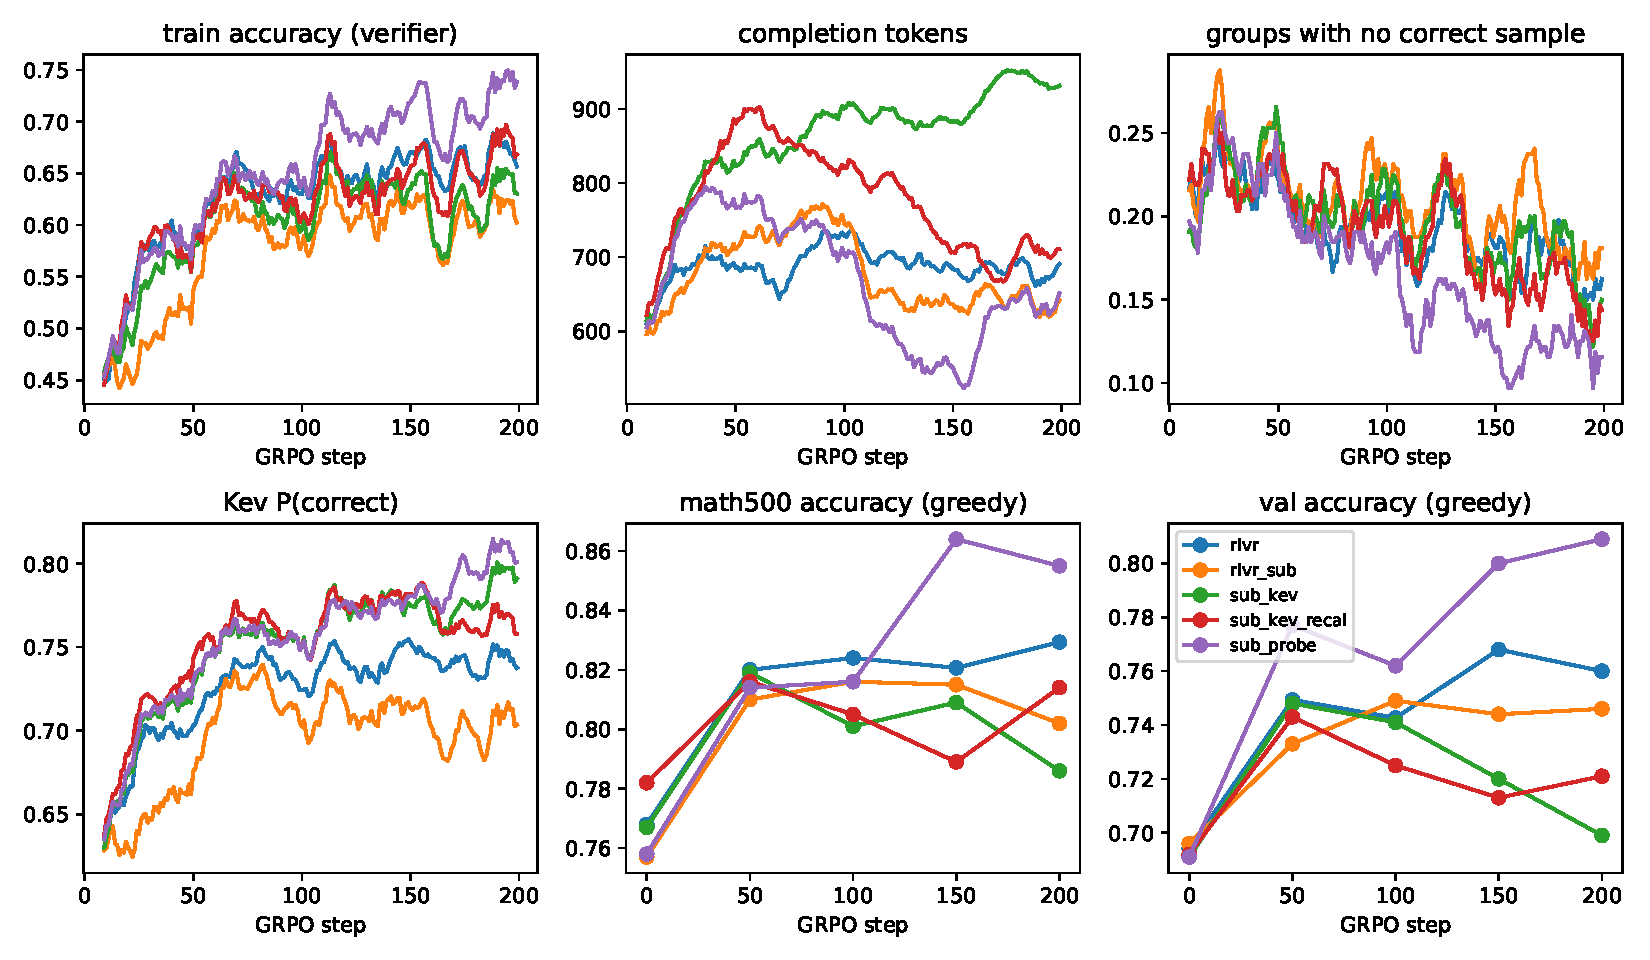
\includegraphics[width=\linewidth]{../../experiments/part3b_labels/results/training_curves.pdf}
\caption{训练曲线（种子均值）：全部训练解答（无论是否标注）的验证器准确率、解答词元数、没有任何正确解答的组所占比例、训练解答上 \kev{} 的 $\pc$（10 步滑动平均），以及每 50 步在 MATH-500 和验证集上的贪心准确率。}
\label{fig:sub-curves}
\end{figure}

\paragraph{评估噪声。} 在本比较的 \NUM{szruns_math500} 个 run 中，基座模型第 0 步的 MATH-500 准确率在 \NUM{szmin_math500}\% 到 \NUM{szmax_math500}\% 之间；一个 run 在第 150 步与第 200 步的评估之间平均变化 \NUM{lecabs_math500} 个百分点。每个 run 的最终权重在 MATH-500 上被贪心评估两次：一次是第 200 步的定期评估，一次是最终评估。两次结果平均相差 \NUM{rptabs_math500} 个百分点，最多相差 \NUM{rptmax_math500}（\NUM{rptruns_math500} 个 run）。

\subsection{先写草稿}\label{sec:res-style}

第二部分发现，有些 GRPO run 会突然切换到这样一种风格：解答先用纯文本、不带 LaTeX 或 markdown 写一份非正式草稿，给出答案，之后常常再写格式化的解答；而发生切换的 run 正是最好的那些。我们用以这种草稿开头的解答所占比例来衡量这一风格（前 300 个字符中没有数学定界符、markdown 标题或粗体；第二部分 \S8.3，在读过解答之后定义）。基座模型的 MATH-500 解答有 \NUM{pdraftat_0_min} 到 \NUM{pdraftat_0_max} 以这种方式开头。

\paragraph{只有探针的策略发生了切换。} 除一个 run 外，每个 run 在前 50 步都压低了草稿的比例（表~\ref{tab:sub-drafts}）。例外是 \texttt{sub\_probe} 种子 1：它在第 50 步有 \NUM{draftat_subprobe_s1_50} 的 MATH-500 解答以草稿开头，第 100 步为 \NUM{draftat_subprobe_s1_100}。\texttt{sub\_probe} 种子 2 的这一比例在第 50 步降到 \NUM{draftat_subprobe_s2_50}，随后上升，从第 100 步的 \NUM{draftat_subprobe_s2_100} 升到第 150 步的 \NUM{draftat_subprobe_s2_150}。标注预算条件的其他六个 run 以及 \texttt{rlvr} 的三个 run，在最终评估中都至多为 \NUM{pdraftmax_other}。在本项目的 \NUM{allruns} 个 GRPO run 中，发生切换的 \NUM{alldraftruns} 个分属 \NUM{alldraftconds} 个不同条件，正是 AIME24 上最好的 \NUM{alldraftruns} 个（\NUM{alldraftaime24min}\% 到 \NUM{alldraftaime24max}\%，其他 run 至多 \NUM{allotheraime24max}\%；第二部分 \S8.3）。\texttt{sub\_probe} 相对 \texttt{rlvr\_sub} 的增益伴随着这一切换；只有两个种子，我们无法把探针的作用与切换的作用分开。

\begin{table}[t]
\centering\small
\begin{tabular}{@{}lccccccccc@{}}
\toprule
& & & & \multicolumn{5}{c}{share of drafts, step} & \\ \cmidrule(lr){5-9}
condition & seed & MATH-500 & AIME24 & 0 & 50 & 100 & 150 & 200 & final \\ \midrule
\texttt{rlvr} & 1 & 82.8 & 21.0 & 12\% & 1\% & 0\% & 1\% & 1\% & 1\% \\
 & 2 & 83.0 & 21.9 & 12\% & 0\% & 0\% & 0\% & 0\% & 0\% \\
 & 3 & 81.8 & 21.7 & 12\% & 1\% & 1\% & 0\% & 1\% & 1\% \\
\addlinespace
\texttt{rlvr\_sub} & 1 & 80.6 & 19.6 & 11\% & 3\% & 1\% & 1\% & 1\% & 1\% \\
 & 2 & 83.0 & 17.1 & 12\% & 3\% & 2\% & 1\% & 2\% & 2\% \\
\addlinespace
\texttt{sub\_kev} & 1 & 78.6 & 14.8 & 11\% & 2\% & 1\% & 1\% & 2\% & 1\% \\
 & 2 & 80.4 & 17.1 & 12\% & 2\% & 1\% & 1\% & 1\% & 2\% \\
\addlinespace
\texttt{sub\_kev\_recal} & 1 & 79.4 & 17.9 & 12\% & 2\% & 1\% & 2\% & 6\% & 7\% \\
 & 2 & 83.0 & 24.4 & 12\% & 1\% & 2\% & 3\% & 1\% & 1\% \\
\addlinespace
\texttt{sub\_probe} & 1 & 87.2 & 30.6 & 12\% & 28\% & 91\% & 98\% & 91\% & 90\% \\
 & 2 & 84.6 & 30.4 & 12\% & 5\% & 9\% & 90\% & 89\% & 90\% \\
\bottomrule
\end{tabular}

\caption{以非正式草稿开头的 MATH-500 解答所占比例：每次定期评估（贪心，每 50 步）和最终评估，逐个 run 列出，并附最终准确率。}
\label{tab:sub-drafts}
\end{table}

\paragraph{补全奖励为草稿付了多少。} 在一组之内，GRPO 偏向奖励更高的解答，因此当一种风格的解答比同组其他解答得到更多回报时，这种风格就会扩散。表~\ref{tab:sub-draftgroups} 按验证器的判定比较草稿与同组其他解答，表~\ref{tab:sub-draftfill} 按判定相同的未标注解答上的补全奖励比较二者。第 0--49 步，在全部 \NUM{pdgn_0} 个 run 中草稿都比同组其他解答更少被判正确（差值在 \NUM{pdgverdict_0_min} 到 \NUM{pdgverdict_0_max} 个百分点之间），这就是它们的比例下降的原因。在 \texttt{sub\_probe} 的两个 run 中，从第 50 步起，草稿被判正确的频率不低于其他解答（种子 1 为 \NUM{dgverdict_subprobe_s1_50} 和 \NUM{dgverdict_subprobe_s1_100} 个百分点，种子 2 为 \NUM{dgverdict_subprobe_s2_50} 和 \NUM{dgverdict_subprobe_s2_100}）；在草稿扩散的那些窗口里，探针给正确草稿的回报高于其他正确解答（种子 1 第 50--99 步高 \NUM{dgfillright_subprobe_s1_50} 个百分点，种子 2 第 50--149 步高 \NUM{dgfillright_subprobe_s2_50} 和 \NUM{dgfillright_subprobe_s2_100}）。其他补全 run 的情况则不一。在 \texttt{sub\_kev\_recal} 种子 2 中，run 的后半段草稿比其他解答更常被判正确（\NUM{dgverdict_subrecal_s2_100} 和 \NUM{dgverdict_subrecal_s2_150} 个百分点），重新校准的输出头却给正确草稿更低的回报（\NUM{dgfillright_subrecal_s2_100} 和 \NUM{dgfillright_subrecal_s2_150}），草稿也没有扩散。在 \texttt{sub\_kev\_recal} 种子 1 中，输出头在第 100--199 步给正确草稿更高的回报（\NUM{dgfillright_subrecal_s1_100} 和 \NUM{dgfillright_subrecal_s1_150}），草稿同样没有扩散。几个 run 的几个窗口、事后读出的结果，说明不了是什么让探针的 run 发生了切换；何况第三部分 C 中也有只用验证器奖励就发生切换的 run（第二部分 \S8.3）。

\begin{table}[t]
\centering\small
\begin{tabular}{@{}lccccccccc@{}}
\toprule
 & & \multicolumn{2}{c}{steps 0--49} & \multicolumn{2}{c}{steps 50--99} & \multicolumn{2}{c}{steps 100--149} & \multicolumn{2}{c}{steps 150--199} \\ \cmidrule(l{2pt}r{2pt}){3-4}\cmidrule(l{2pt}r{2pt}){5-6}\cmidrule(l{2pt}r{2pt}){7-8}\cmidrule(l{2pt}r{2pt}){9-10}
condition & seed & drafts & $\Delta$ right & drafts & $\Delta$ right & drafts & $\Delta$ right & drafts & $\Delta$ right \\ \midrule
\texttt{rlvr} & 1 & 7\% & $-$8.5 & 2\% & $+$4.2 & 1\% & $-$3.9 & 2\% & $+$1.8 \\
 & 2 & 5\% & $-$15.3 & 1\% & $-$9.3 & 0\% & $-$5.0 & 0\% & $-$2.1 \\
 & 3 & 6\% & $-$14.3 & 1\% & $-$0.7 & 1\% & $+$3.3 & 1\% & $+$2.6 \\
\addlinespace
\texttt{rlvr\_sub} & 1 & 13\% & $-$8.3 & 3\% & $-$7.2 & 2\% & $-$5.1 & 1\% & $-$5.5 \\
 & 2 & 11\% & $-$13.7 & 4\% & $-$3.3 & 2\% & $-$10.0 & 4\% & $+$0.2 \\
\addlinespace
\texttt{sub\_kev} & 1 & 10\% & $-$8.9 & 4\% & $-$5.9 & 2\% & $-$5.7 & 3\% & $+$2.8 \\
 & 2 & 12\% & $-$11.0 & 6\% & $-$3.6 & 1\% & $-$8.8 & 1\% & $-$5.0 \\
\addlinespace
\texttt{sub\_kev\_recal} & 1 & 8\% & $-$8.9 & 3\% & $-$2.9 & 2\% & $-$4.0 & 5\% & $+$0.0 \\
 & 2 & 11\% & $-$5.7 & 2\% & $-$0.3 & 3\% & $+$1.6 & 2\% & $+$4.8 \\
\addlinespace
\texttt{sub\_probe} & 1 & 14\% & $-$2.4 & 52\% & $+$1.5 & 94\% & $+$3.8 & 96\% & $+$1.6 \\
 & 2 & 10\% & $-$8.3 & 3\% & $+$1.4 & 56\% & $+$0.6 & 88\% & $+$2.8 \\
\bottomrule
\end{tabular}

\caption{以非正式草稿开头的训练解答，按 50 步的窗口：它们所占比例，以及 $\Delta$ right：在同时含有两类解答的组上取平均的、草稿被验证器判为正确的比例减去同组其他解答的这一比例（百分点）。}
\label{tab:sub-draftgroups}
\end{table}

\begin{table}[t]
\centering\small
\begin{tabular}{@{}lccccccccc@{}}
\toprule
 & & \multicolumn{2}{c}{steps 0--49} & \multicolumn{2}{c}{steps 50--99} & \multicolumn{2}{c}{steps 100--149} & \multicolumn{2}{c}{steps 150--199} \\ \cmidrule(l{2pt}r{2pt}){3-4}\cmidrule(l{2pt}r{2pt}){5-6}\cmidrule(l{2pt}r{2pt}){7-8}\cmidrule(l{2pt}r{2pt}){9-10}
condition & seed & right & wrong & right & wrong & right & wrong & right & wrong \\ \midrule
\texttt{sub\_kev} & 1 & $-$2.5 & $-$1.6 & $+$0.5 & $-$0.7 & $+$0.0 & $-$3.2 & $+$0.0 & $-$2.5 \\
 & 2 & $+$2.2 & $-$1.4 & $-$1.1 & $-$2.2 & $-$1.8 & $-$3.5 & $-$2.4 & $-$1.3 \\
\addlinespace
\texttt{sub\_kev\_recal} & 1 & $-$5.4 & $-$10.4 & $-$0.5 & $+$5.1 & $+$3.6 & $-$4.6 & $+$3.6 & $+$6.3 \\
 & 2 & $-$2.9 & $-$6.0 & $-$0.3 & $-$0.5 & $-$2.5 & $-$4.6 & $-$3.2 & $-$1.3 \\
\addlinespace
\texttt{sub\_probe} & 1 & $+$0.5 & $-$7.0 & $+$2.1 & $-$1.5 & $-$0.4 & $+$10.3 & $+$0.3 & $+$1.4 \\
 & 2 & $-$1.0 & $-$6.7 & $+$5.3 & $-$7.6 & $+$1.9 & $+$3.3 & $-$0.9 & $+$2.1 \\
\bottomrule
\end{tabular}

\caption{以非正式草稿开头的未标注训练解答的补全奖励，减去同组中判定相同（right 或 wrong）的其他未标注解答的补全奖励，按 50 步的窗口，在同时含有两者的组上取平均（百分点）；--- 表示没有这样的组。}
\label{tab:sub-draftfill}
\end{table}

\subsection{评判模型会为重复付费吗？}\label{sec:res-repeat}

GRPO run 结束之后，我们用第二部分的探针（\file{dcjev/llm/repeat_probe.py}；表~\ref{tab:repeat-probe}）检验了 \kev{} 是否会为 \texttt{sub\_kev} 和 \texttt{sub\_kev\_recal} 的策略在第一个答案之后所写的内容付费。\texttt{sub\_kev} 的种子 1 一遍又一遍地重述结论；\texttt{sub\_kev\_recal} 的种子 1 用几乎相同的话把题目再解一遍，就像第二部分中重复的策略那样。我们把种子 1 在第一个答案之后出现重复行的最终 MATH-500 解答截断在第一个答案处，就像策略在那里停下了一样。在第一个答案之前就开始重复的解答，以及第一个答案与最后一个答案不同的解答，不计在内（分别 \NUM{rpskip_subkev} 和 \NUM{rpskip_subrecal} 个）。所有改动都不改变验证器读到的答案。

第一个答案之后的部分让发布版 \kev{} 的 $\pc$（也就是 \texttt{sub\_kev} 的补全奖励）在正确答案上提高 \NUM{rpkevc_cutsubkev_1} \ci{\NUM{rpkevclo_cutsubkev_1}}{\NUM{rpkevchi_cutsubkev_1}}，在错误答案上提高 \NUM{rpkevc_cutsubkev_0} \ci{\NUM{rpkevclo_cutsubkev_0}}{\NUM{rpkevchi_cutsubkev_0}}。在 \texttt{sub\_kev\_recal} 的解答上，它提高 \NUM{rpkevc_cutsubrecal_1} \ci{\NUM{rpkevclo_cutsubrecal_1}}{\NUM{rpkevchi_cutsubrecal_1}} 和 \NUM{rpkevc_cutsubrecal_0} \ci{\NUM{rpkevclo_cutsubrecal_0}}{\NUM{rpkevchi_cutsubrecal_0}}，\NUM{rpkevcup_cutsubrecal_0} 的错误答案分数上升。单纯的重复价值不大：写进基座策略的解答时，它让 \kev{} 的 $\pc$ 在正确答案上提高 \NUM{rpkevc_end3_1}，在错误答案上变化 \NUM{rpkevc_end3_0}。所以在未标注的解答上，补全奖励为这些策略在第一个答案之后学会写的内容付了费，在错误答案上尤其如此——而验证器对这些错误答案本不会给任何回报。探针用发布版输出头打分；\texttt{sub\_kev\_recal} 的输出头在训练中被重新拟合过，它在 run 结束时自己的偏好这里没有测量。没有任何条件用到的 AR 评判模型，给带有第一个答案之后部分的 \texttt{sub\_kev\_recal} 解答打更高的分（正确答案上 \NUM{rparc_cutsubrecal_1}），却给 \texttt{sub\_kev} 无休止的重述打更低的分（正确答案上 \NUM{rparc_cutsubkev_1}，错误答案上 \NUM{rparc_cutsubkev_0}）。

\begin{table}[t]
\centering\small\setlength{\tabcolsep}{5pt}
\begin{tabular}{@{}lccccccc@{}}
\toprule
 & solutions & \multicolumn{2}{c}{\kev{} $\pc$} & \multicolumn{2}{c}{\kev{} $\pg$} & \multicolumn{2}{c}{AR $P_{\mathrm{a}}$} \\ \cmidrule(lr){3-4}\cmidrule(lr){5-6}\cmidrule(l){7-8}
 & right / wrong & right & wrong & right & wrong & right & wrong \\ \midrule
\multicolumn{8}{@{}l}{\emph{base policy's solutions, repetition added}} \\
\quad last two paragraphs twice more & 2436 / 1537 & $+$0.012 & $-$0.002 & $+$0.007 & $-$0.006 & $+$0.037 & $+$0.012 \\
\quad written twice & 2436 / 1564 & $+$0.012 & $-$0.003 & $+$0.006 & $-$0.004 & $+$0.029 & $+$0.007 \\
\multicolumn{8}{@{}l}{\emph{repeating final solutions of GRPO runs, as written against cut after the first answer}} \\
\quad \texttt{sub\_kev}, seed 1 & 351 / 66 & $+$0.031 & $+$0.049 & $+$0.016 & $+$0.031 & $-$0.018 & $-$0.074 \\
\quad \texttt{sub\_kev\_recal}, seed 1 & 318 / 81 & $+$0.059 & $+$0.110 & $+$0.030 & $+$0.095 & $+$0.034 & $+$0.034 \\
\bottomrule
\end{tabular}

\caption{重复对评判模型值多少（第二部分的探针）：P（有重复）减 P（无重复），分别在验证器判为正确（right）和错误（wrong）的解答上，附各自的数量。上：第二部分判断研究中基座策略的解答，加入重复。下：种子 1 中含重复行的最终 MATH-500 解答，原样对比在第一个答案之后截断。发布版 \kev{} 的 $\pc$ 和 $\pg$ 以及 AR 评判模型的 $P_{\mathrm{a}}$；正文中的区间按题目重采样。}
\label{tab:repeat-probe}
\end{table}
